\documentclass{standalone}
\usepackage{tkz-base}
\usepackage{tkz-fct}
\usepackage{tkz-euclide}
\usepackage{tikz}
\usetikzlibrary{intersections}
\begin{document}
    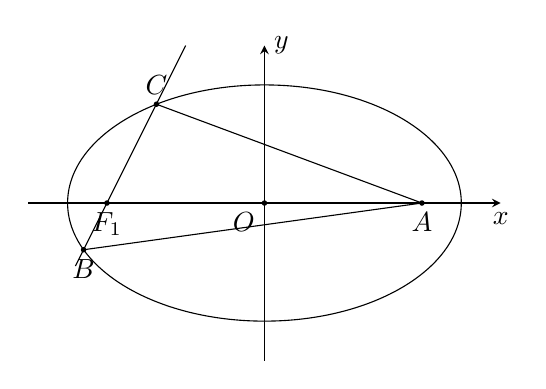
\begin{tikzpicture}
        \pgfmathsetmacro\x{3}
        \pgfmathsetmacro\y{2}
        \pgfmathsetmacro\a{2.5}
        \pgfmathsetmacro\b{1.5}
        \pgfmathsetmacro\c{sqrt(abs(\a^2-\b^2))}
        \coordinate (O) at (0,0);
        \coordinate (F1) at (-\c,0);
        \coordinate (F2) at (\c,0);
        \draw[-stealth] (-\x,0) -- (\x,0) node [below] {$x$};
        \draw[-stealth] (0,-\y) -- (0,\y) node [right] {$y$};
        \fill (O) node [below left] {$O$} circle (1pt);
        \fill (F1) node [below] {$F_1$} circle (1pt);
        \fill (F2) node [below] {$A$} circle (1pt);
        \coordinate (I) at (-1,2);
        \coordinate (J) at ($(F1)!-0.4!(I)$);
        \draw[name path = a] (O) circle [x radius=\a,y radius=\b];
        \draw[name path = b] (I) -- (J);
        \fill [name intersections={of=a and b,by={A,B}}]
        (A) circle (1pt) node [above] {$C$}
        (B) circle (1pt) node [below] {$B$};
        \draw (A) -- (F2) -- (B);
    \end{tikzpicture}
\end{document}